\documentclass[conference,compsoc]{IEEEtran}

\usepackage[utf8]{inputenc}
\usepackage[T1]{fontenc}
\DeclareUnicodeCharacter{0394}{\ensuremath{\Delta}}
\usepackage{amsmath, amssymb, amsthm}
\usepackage{graphicx}
\usepackage{hyperref}
\usepackage{cite}
\usepackage{xcolor}
\usepackage{booktabs}
\usepackage{array}
\usepackage{algorithm}
\usepackage{algpseudocode}
\usepackage{listings}
\usepackage{url}

\newtheorem{theorem}{Theorem}
\newtheorem{lemma}[theorem]{Lemma}
\newtheorem{definition}[theorem]{Definition}

\newcommand{\todoPI}[1]{\textcolor{red}{[PI: #1]}}

% =====================================================================
% Macros for revision-pass numbers; backfilled from the JSON outputs
% (mission_3b/results/) once the corresponding campaigns complete. Each
% line documents the source file the value comes from for audit.
% =====================================================================
% --- Per-style FPR on extended (>=200 paraphrase) corpus ---
% per_style_canonical_extended_qwen3.json
\newcommand{\extPerStyleN}{227}
\newcommand{\extPerStyleFPR}{$1/227 = 0.44\%$}
\newcommand{\extPerStyleCI}{$[0.08, 2.45]$}
% --- T2 probes extended (>=30 prompts) ---
% t2_probes_extended_qwen3.json
\newcommand{\tTwoN}{31}
\newcommand{\tTwoCorrect}{25/31}
\newcommand{\tTwoCorrectPct}{80.6}
% --- MSB subset evaluation (canonical PG-DSL + MCPShield) ---
% msb_subset_evaluation.json
\newcommand{\msbNCpgdsl}{6/8 (75\%, CI [41, 93])}
\newcommand{\msbNCmcpshield}{2/8 (25\%, CI [7, 59])}
\newcommand{\msbPMpgdsl}{1/8 (12\%, CI [2, 47])}
\newcommand{\msbPMmcpshield}{0/8 (0\%, CI [0, 32])}
\newcommand{\msbPIpgdsl}{0/8 (0\%, CI [0, 32])}
\newcommand{\msbPImcpshield}{0/8 (0\%, CI [0, 32])}
\newcommand{\msbOPpgdsl}{1/8 (12\%, CI [2, 47])}
\newcommand{\msbOPmcpshield}{0/8 (0\%, CI [0, 32])}
\newcommand{\msbZthreepgdsl}{1/1 (100\%)}
\newcommand{\msbZthreemcpshield}{0/1 (0\%)}
% --- Real-agent N=10 campaign aggregate ---
% real_agent_asr_n10.json
\newcommand{\realAgentAonewithout}{$10/10 = 100\%$ $[72.2, 100.0]$}
\newcommand{\realAgentAonewith}{$0/10 = 0\%$ $[0.0, 27.8]$}
\newcommand{\realAgentAtwowithout}{$0/10 = 0\%$ $[0.0, 27.8]$}
\newcommand{\realAgentAtwowith}{$0/10 = 0\%$ $[0.0, 27.8]$}
\newcommand{\realAgentWtwowithout}{$9/10 = 90\%$ $[59.6, 98.2]$}
\newcommand{\realAgentWtwowith}{$9/10 = 90\%$ $[59.6, 98.2]$}
\newcommand{\realAgentAtwoengwithout}{$5/10 = 50\%$ $[23.7, 76.3]$}
\newcommand{\realAgentAtwoengwith}{$0/10 = 0\%$ $[0.0, 27.8]$}
\newcommand{\perStyleFormal}{0/84 (0.00\%, CI $[0.00, 4.37]$)}
\newcommand{\perStyleCasual}{1/77 (1.30\%, CI $[0.23, 7.00]$)}
\newcommand{\perStyleTerse}{0/66 (0.00\%, CI $[0.00, 5.50]$)}
\newcommand{\perStyleSeed}{0/42 (0.00\%)}
\newcommand{\perStyleMistral}{1/185 (0.54\%)}

\title{{PG-DSL}: Physics-Grounded Description Lifting for
       Admission-Time Defence of {LLM}-Controlled Industrial
       Cyber-Physical Systems}

% Double-blind submission --- anonymized author block.
\author{\IEEEauthorblockN{Anonymous Authors}
        \IEEEauthorblockA{}}

\begin{document}
\maketitle

\begin{abstract}
LLM agents increasingly control industrial cyber-physical systems via
the Model Context Protocol (MCP), inheriting a description channel
the agent cannot verify: the natural-language tool description is
read at discovery time and shapes plan-time choices.
Description-poisoning attacks~\cite{mcp_misleading,when_mcp_attack}
and real-world
incidents~\cite{dragos_mexico_26} demonstrate the channel is
operationally exploited. We present \textbf{PG-DSL} (Physics-Grounded
Description Lifting), an admission-time defence that lifts each tool
description into a formal claim over a CPS-grounded grammar, replays
the tool against a digital twin (DT), and admits only tools whose
claimed effect matches DT-measured behaviour. PG-DSL verifies a
narrower object than full agent verification
(undecidable~\cite{trust_auth_sok}) or LLM-as-judge verification
(manipulable~\cite{gaming_judge}): the bounded tool implementation
under DT replay, subject to the fidelity bounds of the modeled CPS
dynamics. We formalize three conditional properties under bounded DT
fidelity and a restricted grammar: T1${}_v$, a vectorized detection
threshold; T2, a lifting-soundness decomposition; T3, a
strict-composition witness on a canonical attack set, showing
admission-time and runtime defences cover complementary visibility
surfaces.
On a SWaT P1+P2 substrate with $14$ MCP tools and an $8$-attack
canonical set, PG-DSL achieves $0/42$ benign per-tool admission
rejections ($0.00\%$ FPR, Wilson 95\%~CI~$[0.00\%, 8.38\%]$) and
$0.44\%$ per-style FPR (CI~$[0.08\%, 2.45\%]$) on a $227$-paraphrase
corpus generated by an out-of-family paraphraser. PG-DSL alone blocks
$6/8$ attacks at admission; the remaining two ($W_1, W_2$) are
intentionally outside admission-time scope. Composed with
INVARLLM~\cite{invarllm}, the union covers all $8$. We release a
digital-twin-replicable artifact and a provenance map.
\end{abstract}

\IEEEpeerreviewmaketitle

\section{Introduction}
\label{sec:intro}
% =====================================================================

Recent measurement work on Model Context Protocol
servers~\cite{mcp_misleading} found that approximately $13\%$ of
real-world MCP servers exhibit description--code mismatches sufficient
to enable unauthorised actions when an LLM agent reads the description
verbatim. Concurrent threat intelligence from
Dragos~\cite{dragos_mexico_26} reported the use of large language
models in an intrusion campaign against a municipal water and drainage
utility serving the Monterrey metropolitan area, with the LLM
identified as the primary technical executor of operational-technology
reconnaissance during the December~2025--February~2026 window.
Together these data points establish a threat class with operational
presence: \emph{description-channel poisoning} of LLM-controlled
industrial cyber-physical systems.

\paragraph{Why classical defences do not apply.}
Two recent results constrain the design space. First, the
trust-authorisation mismatch SoK~\cite{trust_auth_sok} invokes Rice's
theorem to argue that semantic verification of a Turing-complete agent
is undecidable; static access-control mechanisms are
\emph{structurally} incapable of governing probabilistic agent
behaviour. Second, ``Gaming the Judge''~\cite{gaming_judge} shows that
LLM-as-judge verifiers can be manipulated by chain-of-thought adversaries,
with empirical false-positive rates up to $90\%$ on adversarially
constructed inputs. Together these results rule out (i) static
verification of the agent itself and (ii) LLM-on-LLM verification.

\paragraph{The PG-DSL approach.}
We avoid both limitations by narrowing what is verified and what
verifies it. Instead of verifying the \emph{agent}, PG-DSL verifies
each \emph{tool}: a tool is a bounded computational artifact whose
physical effect in a digital twin is decidable up to a fidelity bound
$\varepsilon_{DT}$. Instead of using another LLM to judge truthfulness,
PG-DSL uses physics: a discrete-time mass-balance digital twin
serves as the verifier substrate. Each natural-language tool
description is lifted to a formal claim $\varphi$ over a CPS-grounded
grammar of actuators, sensors, and state-variable
deltas; the claim is checked against a measured trajectory $\psi$ from
the DT before the agent ever observes the tool. Tools whose claimed
and measured effects diverge are rejected from the agent's catalog.

The defence is \emph{admission-time} (per-tool, before context
injection) and is composition-aware: the same matcher that checks
single-tool descriptions is applied to ordered pairs of admitted tools
to rule out runtime compositions whose joint physical effect breaches
a safety predicate that no constituent tool alone violates.

\paragraph{Contributions.}
This work makes the following contributions:
\begin{itemize}
\item \textbf{Problem formulation.} We frame
      description--implementation mismatch as the load-bearing attack
      surface for MCP-controlled CPS tools, distinct from
      agent-behavior verification (undecidable) and LLM-judge
      defences (manipulable on description content).
\item \textbf{System.} The PG-DSL admission pipeline:
      lifter $L_{\text{verify}}$ (LLM under a restricted CPS-grounded
      grammar, prompt v1 with rules R1--R5), per-tool DT verifier,
      composition-aware DT verifier producing a blocked-pair set for
      runtime enforcement, and formal matcher. All four components
      are instantiated on a SWaT P1+P2 substrate with $14$ MCP tools
      via a real-MCP server consumable by the official Python MCP
      SDK.
\item \textbf{Conditional analysis.} Three properties under bounded
      DT fidelity and a restricted grammar class $\mathcal{C}$:
      T1${}_v$, a vectorized detection threshold $\delta^{*}_v =
      2\,\|\varepsilon_{L,v} + \varepsilon_{DT,v}\|_\infty$ above which
      bounded-error detection is deterministic; T2, a
      lifting-soundness decomposition with empirically estimated
      $\delta_{\text{lift}} = 0.44\%$ on a $227$-paraphrase
      out-of-family corpus (Wilson 95\%~CI~$[0.08\%, 2.45\%]$); T3,
      a witnessed strict-superset property over a canonical
      $8$-attack set with concrete witnesses $A_2 \in
      A_{\text{static}} \setminus A_{\text{runtime}}$ and
      $W_1, W_2 \in A_{\text{runtime}} \setminus A_{\text{static}}$.
\item \textbf{Evaluation.} Canonical PG-DSL alone blocks $6/8$ attacks
      at admission; composed with INVARLLM the union covers all $8$.
      A $\geq 30$-prompt T2 adversarial probe battery and an MSB
      cross-benchmark adaptation establish where PG-DSL is strong
      (description--physics gaps, name collisions, composition) and
      where it has known limits (read-tool sensor aliasing, prompt
      injection embedded in description text). A real-agent campaign
      ($N=10$ operational-condition trials per cell) on
      \texttt{qwen3:14b} demonstrates one end-to-end
      description-poisoning exploit that PG-DSL blocks before
      catalog exposure, and confirms that post-admission spoofing
      remains outside the admission-time scope.
\item \textbf{Artifact.} Digital-twin-replicable Python implementation
      with deterministic stub and \texttt{qwen3:14b} configurations,
      complete provenance map linking every paper claim to its
      primary JSON output and source file.
\end{itemize}

The paper is organised as follows.
\S\ref{sec:background} fixes the protocol-level model, the SWaT
P1+P2 substrate, and the formal preliminaries the theorems build on.
\S\ref{sec:threat} fixes the threat model.
\S\ref{sec:design} states T1${}_v$, T2, T3 with proofs and concrete
witnesses, and describes the canonical PG-DSL pipeline (lifter,
per-tool and composition-aware DT verifiers, formal matcher) plus
implementation footprint.
\S\ref{sec:eval} reports empirical results.
\S\ref{sec:disc} discusses limitations and design implications.
\S\ref{sec:related} positions PG-DSL against MCP defences, runtime
CPS-IDS, contract-grounded tool execution, and NL-to-formal lifting.
\S\ref{sec:conc} concludes.

% =====================================================================

\section{Background}
\label{sec:background}
% =====================================================================

We fix the protocol-level model, the substrate, the formal
preliminaries the theorems build on, and the runtime-CPS-IDS baseline
the T3 composition pairs with. Readers familiar with the Model
Context Protocol and the SWaT testbed may skim this section.

\subsection{Model Context Protocol (MCP) and Tool Admission}

An MCP server exposes a finite set of \emph{tools}; each tool is a
triple $\mathcal{T} = (\mathit{name}, \mathit{description},
\mathit{impl})$, where $\mathit{description}$ is natural-language
text consumed at \emph{discovery time} by the agent (as part of the
agent's prompt context) and $\mathit{impl}$ is the executable callback
that runs when the agent invokes the tool by name. Per the official
specification~\cite{mcp_spec}, the agent's session begins with a
\texttt{tools/list} request that returns the tool catalog; the agent
then issues \texttt{tools/call} requests that route through
$\mathit{impl}$.
PG-DSL inserts an \emph{admission gate} between the server and the
agent's catalog view: the gate consumes
$(\mathit{description}_i, \mathit{impl}_i)$ for each tool $i$, runs a
digital-twin replay of $\mathit{impl}_i$, lifts
$\mathit{description}_i$ to a formal claim $\varphi_i$, and either
admits the tool (the agent sees it) or rejects it (the agent's catalog
does not contain it).

\subsection{Description-Channel Poisoning}

A \emph{description-channel poisoning} attack constructs a triple
$(\mathit{name}, \mathit{description}', \mathit{impl}')$ such that
$\mathit{description}'$ encodes claims an LLM agent will rely on to
choose the tool, while $\mathit{impl}'$'s observable effect on the
plant diverges from those claims --- either because
$\mathit{description}'$ misrepresents
the actuator/sensor relationship (type confusion, sensor aliasing),
or because $\mathit{description}'$ misrepresents the parametric
semantics (magnitude poisoning), or because the divergence emerges
from joint behaviour of multiple admitted tools (composition).
The attack class is operationally exploited in the wild: recent
measurement work~\cite{mcp_misleading} reports approximately $13\%$
of real-world MCP servers exhibit description--code mismatches, and
field threat intelligence~\cite{dragos_mexico_26} attributes the
December~2025--February~2026 Monterrey water-utility incident to
LLM-controlled tool invocation against operational supervisory
systems.

\subsection{SWaT P1+P2 Substrate}

We evaluate PG-DSL on a digital twin of the SWaT industrial
water-treatment testbed at iTrust SUTD, restricted to Process Stages
P1 (raw-water intake) and P2 (chemical dosing). The substrate has:
$2$ raw-water tanks (T101 the inflow buffer, T201 the dosing buffer);
$2$ motorised inlet valves (MV101 between the supply manifold and
T101; MV201 between T101 and the P2 dosing line); $2$ raw-water
pumps (P101, P102 feeding T101); $6$ chemical dosing pumps (P201
through P206 dosing the P2 line); and $7$ analyser sensors (LIT101,
LIT201 measuring tank levels; FIT101, FIT201 measuring flows;
AIT201--AIT203 measuring chemistry). The MCP server exposes $14$
canonical tools $\{\texttt{open\_valve\_MV101},
\texttt{close\_valve\_MV101}, \texttt{start\_pump\_P101},
\texttt{stop\_pump\_P101}, \texttt{open\_valve\_MV201},
\texttt{close\_valve\_MV201},$ $\texttt{start\_dosing\_pump\_P201},$
$\texttt{stop\_dosing\_pump\_P201},$
$\texttt{set\_dosing\_rate}, \texttt{read\_level\_T101},$
$\texttt{read\_level\_T201}, \texttt{read\_flow\_FIT101},$
$\texttt{read\_flow\_FIT201}, \texttt{read\_chemical\_AIT201}\}$.
Plant dynamics are mass balance plus linearised
chemistry~\cite{minicps}: tank levels evolve as $\dot L_T = q_{\text{in}}
- q_{\text{out}}$ conditional on valve and pump state; chemistry
follows a linearised-Cond model in the operating band.

\subsection{Formal Preliminaries}

\paragraph{Sensing and lifting errors.}
The lifter $L_{\text{verify}}: \mathcal{C} \to \Phi$ maps
descriptions in a structured grammar $\mathcal{C}$ to formal claims
$\varphi$ over actuators, sensors, and state-variable deltas. We
assume \emph{bounded semantic error} on $\mathcal{C}$: there exists
$\varepsilon_L$ such that $\sup_{D \in \mathcal{C}}
\|L_{\text{verify}}(D) - \varphi^{*}(D)\| \leq \varepsilon_L$, where
$\varphi^{*}(D)$ is the ground-truth claim and $\|\cdot\|$ is a
semantic distance over claims (we instantiate this as per-sample
bias in sensor space). The digital twin $\mathit{DT}$ has \emph{bounded
per-sample fidelity error} $\varepsilon_{DT}$: for any trajectory
$\psi^*$ on the real plant and matching $\psi$ on $\mathit{DT}$,
$\sup_t \|\psi(t) - \psi^*(t)\| \leq \varepsilon_{DT}$.

\paragraph{Vectorized state.}
The relevant physical state space is $\Sigma \subseteq \mathbb{R}^n$
with $n=2$ on SWaT P1+P2: $(L_{T101}, L_{T201})$ at admission time.
Per-coordinate sensing and lifting errors are
$\varepsilon_{L,v}, \varepsilon_{DT,v} \in \mathbb{R}^n$.

\subsection{Runtime CPS-IDS Baseline (INVARLLM)}

The runtime composition partner in T3 is INVARLLM~\cite{invarllm}: a
classical CPS-IDS that extracts physical invariants from benign
trajectories (mass-balance, sensor-redundancy, monotonicity) and
fires when an online trajectory violates a learned invariant.
INVARLLM has admission-time blindness by construction: it observes
runtime telemetry, not tool descriptions. Composed with PG-DSL,
INVARLLM provides the runtime layer that closes the
$A_{\text{runtime}} \setminus A_{\text{static}}$ direction of T3
(\S\ref{sec:design}).

% =====================================================================

\section{Threat Model}
\label{sec:threat}
% =====================================================================

\paragraph{System.}
An LLM agent $A$ controls a CPS plant $P$ (water-treatment substrate
SWaT P1+P2, with raw-water intake T101, chemical-dosing buffer T201,
transfer valves $\{$MV101, MV201$\}$, raw-water pumps
$\{$P101, P102$\}$, dosing pumps $\{$P201--P206$\}$, and analyser
sensors $\{$LIT101, LIT201, FIT101, FIT201, AIT201--AIT203$\}$). The
agent issues actions to $P$ via Model Context
Protocol~\cite{mcp_spec} \emph{tool calls}: each tool exposes a
natural-language description, an input schema, and an
implementation that wraps a PLC-style command on $P$. The defender
places a physics-grounded verifier $V$ between the MCP server and
$A$'s tool catalog.

\paragraph{Attacker.}
The attacker controls the natural-language description of one or more
MCP tools, the implementation behind those tools, or both, and can
optionally pre-set the physical actuator state on $P$ before the
agent's session begins. The attacker may additionally spoof sensor
reads at the network layer (post-admission). The attacker cannot
modify the verifier $V$, the digital twin $\mathit{DT}$, the lifter
$L_{\text{verify}}$, or the formal matcher; nor can the attacker
bypass the admission gate.

\paragraph{Attack classes.}
We organise attacks into three categories aligned with the empirical
campaigns.
\begin{enumerate}
\item \textbf{Description-poisoning} (A1, A2, A3): the attacker writes
      a description that mismatches the tool's implementation. A1 is
      type-confusion (the description claims a tool drains while the
      implementation fills); A2 is magnitude poisoning on a parametric
      tool (the description names a unit/scale that the
      implementation does not honour); A3 is sensor aliasing (the
      description claims one sensor while the implementation returns
      another).
\item \textbf{Composition} (Z1, Z2, Z3): the attack manifests through
      the joint behaviour of multiple individually-admitted tools.
      Z1 is a single-tool transient overshoot exploiting steady-state
      semantics in the lifted band; Z2 is overdose magnitude poisoning
      (mirror of A2); Z3 is the canonical strict-composition witness
      (described in detail in \S\ref{sec:t3-witnesses}).
\item \textbf{Runtime} (W1, W2): the attack is invisible at admission
      time and manifests after the agent's session begins. W1 is a
      sub-noise-floor stealth drain that respects the description's
      claimed state-zero invariant within per-sample fidelity but
      accumulates a cumulative drift exceeding the matcher's
      cumulative budget. W2 is post-admission sensor spoofing of
      LIT101 while pumps drive the tank to overflow.
\end{enumerate}

\paragraph{Trusted computing base.}
Table~\ref{tbl:tcb} summarises the trusted computing base. PG-DSL is
only as good as DT fidelity, grammar coverage, and the lifter's
bounded semantic error on $\mathcal{C}$.

\begin{table}[t]
\centering
\footnotesize
\caption{Trusted computing base for PG-DSL. PG-DSL provides no
defence if a trusted component is itself compromised.}
\label{tbl:tcb}
\begin{tabular}{@{}p{0.30\columnwidth}p{0.18\columnwidth}p{0.40\columnwidth}@{}}
\toprule
Component & Trusted? & Rationale \\
\midrule
MCP description & No & attacker-controlled \\
Tool impl. & Partial & may be poisoned; DT observes \\
Digital twin & Yes & verifier substrate, fidelity-bounded \\
Lifter & Yes, fallible & bounded $\varepsilon_L$; T2 quantifies \\
Formal matcher & Yes & deterministic check \\
Runtime telemetry & Partial & W2 spoofs post-admission reads \\
Runtime IDS & Separate & T3 composition partner \\
\bottomrule
\end{tabular}
\end{table}

\paragraph{Out of scope.}
Network-level attacks against the verifier itself, hardware ageing,
chemistry kinetics beyond linearised conductivity, and side-channel
attacks on $L_{\text{verify}}$ (e.g., adversarial probes designed
specifically against the lifter's training distribution) are out of
scope for this paper. These are deferred to T3's runtime composition
partner or to future work.

\paragraph{Real-agent threat realisation.}
A bounded real-agent campaign on the SWaT P1+P2 substrate validates
the threat-model claim end-to-end: a \texttt{qwen3:14b} agent
operating against a real-MCP server via the official Python MCP SDK
falls to description-channel poisoning (A1, type-confusion overflow)
in $10/10$ replications without defence; remains vulnerable to
post-admission sensor spoofing (W2) in $9/10$ replications regardless
of admission-time defence (W2 is a canonical $A_{\text{runtime}}$
witness whose visibility surface is runtime telemetry rather than
admission-time descriptions). With
canonical PG-DSL admission applied, A1 ASR drops to the with-defence
row of Table~\ref{tbl:real-agent-asr} --- the admission gate excludes
the poisoned tool from the agent's catalog before the agent is ever
exposed to the description --- while W2 ASR is unchanged, as
predicted by the T3 partition (W2 is a canonical $A_{\text{runtime}}$
witness). The campaign uses $N=10$ reps $\times$ $30$-step horizons
$\times$ four conditions $\{A_1, A_2, W_2, A_2^{\text{eng}}\}$ at
$10$~s simulated plant-tick per agent action; reps sweep across
realistic operating-condition variation (see \S\ref{sec:eval-real-agent}),
not stochastic LLM-policy independence. Full per-rep traces and
aggregate Wilson~95\% CIs are in the artifact. Detailed numbers
appear in \S\ref{sec:eval-real-agent}.

% =====================================================================

\section{System Design}
\label{sec:design}
\label{sec:theory}
\label{sec:method}
% =====================================================================
% Merged from the prior \S4 Theoretical Framework and \S5 Methodology
% per the polish-pass M3(b) merge decision. Flattened to normal
% subsections per pre-submission review (avoids the prior "4.0.1"
% subsubsection numbering anomaly). All original cross-reference
% labels (sec:theory, sec:method, sec:t3-witnesses,
% sec:dt-calibration, sec:method-grammar) are preserved.
% =====================================================================

The canonical PG-DSL pipeline comprises four components that run as
a single pre-context-injection pass: (i) the \emph{lifter}
$L_{\text{verify}}$, (ii) the \emph{per-tool DT verifier}, (iii) the
\emph{composition-aware DT verifier} (which produces a blocked-pair
set later enforced by a runtime pair guard), and (iv) the
\emph{formal matcher}. Only tools whose claims survive both the
per-tool and composition verifications are exposed to the agent. The
remaining subsections describe each component and the three
conditional properties of the pipeline under bounded DT fidelity and
restricted grammar coverage --- T2 with the lifter (\S\ref{sec:design-lifter}),
T1${}_v$ with the per-tool DT verifier (\S\ref{sec:design-dt}), and
T3 with the composed defence (\S\ref{sec:design-t3}).

\subsection{Class $\mathcal{C}$ of CPS-Grounded Tool Descriptions}
\label{sec:method-grammar}

A description $D \in \mathcal{C}$ is a finite sequence of statements
drawn from the grammar
\[
\begin{aligned}
\text{statement} ::= {}&
  \text{actuator}(\textit{name}) := \textit{value} \\
&\mid\ \text{sensor}(\textit{name})\ \text{reads}\ \textit{value} \\
&\mid\ \Delta\text{state}(\textit{var})\ \{\textit{property}^{+}\}
\end{aligned}
\]
where $\textit{name}$ ranges over the SWaT P1+P2 vocabulary
(MV101, MV201, P101--P206, LIT101, FIT101, and AIT201--AIT203),
$\textit{value}$ over discrete actuator states or numeric sensor
readings, and $\textit{property}$ over monotone~$[\pm]$,
bounded~$[a, b]$, and sign~$[\pm 0]$. The grammar is locked for the
paper; the full Lark grammar is in Appendix~\ref{app:grammar}.

\subsection{Lifter $L_{\text{verify}}$ and T2 Lifting Soundness}
\label{sec:design-lifter}

\paragraph{Lifter.}
$L_{\text{verify}}$ is a locked LLM (\texttt{qwen3:14b} via Ollama at
\texttt{temperature}~$=0.0$, \texttt{seed}~$=42$, \texttt{think}~$=
\text{False}$ to disable thinking-mode token expenditure). The
\texttt{seed} is fixed for environment reproducibility; with $T=0$
and \texttt{think=False} the lifter is deterministic on a fixed
prompt and the seed value has no effect on the output token
distribution. The lifter prompt (``v1''/restrained) instructs the
model to lift \emph{only} explicit content from the description under
five restraint rules R1--R5 (Appendix~\ref{app:prompt}):
explicit-content-only, no-inferred-$\Delta$state, per-clause-lifting,
single-actuator-per-tool, and parametric-tool-minimal. R3--R5 were
added in the revision pass to close failure modes (co-actuator
inference, multi-pump enumeration) surfaced by the extended
out-of-family paraphrase corpus; the artifact ships both v1 variants
for ablation.

We define
\[
\varepsilon_L := \sup_{D \in \mathcal{C}} d\!\left(L_{\text{verify}}(D),
                                                 \varphi^{*}(D)\right),
\]
where $\varphi^{*}(D)$ is the ground-truth claim and $d(\cdot, \cdot)$
is a semantic distance over claims realised in sensor space as the
per-sample bias the lifter induces on the predicted trajectory.

\paragraph{T2 --- Lifting soundness decomposition.}
\begin{theorem}[T2, Lifting Soundness on Class $\mathcal{C}$]
\label{thm:t2}
For tool descriptions $D$ drawn i.i.d.\ from a distribution supported
on $\mathcal{C}$, the verifier LLM $L_{\text{verify}}$ produces a
sound formal claim with probability at least
$1 - \delta_{\text{lift}}$, where
\[
\delta_{\text{lift}}
\;\leq\;
\delta_{\text{cov}}(\mathcal{C}, L_{\text{verify}})
+ \delta_{\text{gram}}(\mathcal{C}),
\]
$\delta_{\text{cov}}$ is the LLM's error rate on $\mathcal{C}$ and
$\delta_{\text{gram}}$ is the rate at which honest descriptions fail
to admit any in-grammar lifting.
\end{theorem}

T2 is parametric in $\delta_{\text{lift}}$: the bound is a structural
decomposition rather than a numerical claim. Empirically, on
\texttt{qwen3:14b} with prompt v1 against a $227$-paraphrase benign
corpus (FORMAL/CASUAL/TERSE styles, generated by an out-of-family
paraphraser \texttt{mistral:7b}), we observe $\delta_{\text{lift}} =
0.44\%$ point estimate (Wilson 95\%~CI~$[0.08\%, 2.45\%]$); a single
CASUAL out-of-grammar rejection out of $227$ entries is the only
rejection. This is well within Req2LTL's prior estimate of
$\sim 11.6\%$ and tighter than the prior $42$-paraphrase corpus.

\subsection{Per-Tool DT Verifier and T1${}_v$ Detection Threshold}
\label{sec:design-dt}

\paragraph{Per-tool DT verifier.}
For each candidate tool, the DT verifier instantiates a fresh
\texttt{SwatP1P2Plant} digital twin~\cite{minicps} with the canonical
$14$-tool surface, sets one of three representative initial states
$\{\text{LOW}, \text{MID}, \text{HIGH}\}$ that sweep the operating
envelope, executes the candidate tool's implementation, and records
the trajectory $\psi$ over a $120$~s admission window. The matcher
checks $\varphi \models \psi$ per state-variable; a mismatch on any
of the three initial states rejects the tool from admission.

\paragraph{Notation.}
Let $\Sigma \subseteq \mathbb{R}^n$ denote the physical state space
relevant to admission verification, with state coordinates indexed by
$k \in \{1, \dots, n\}$. For the canonical SWaT P1+P2 substrate, the
level coordinates of interest at admission time are $(L_{T101},
L_{T201})$ ($n=2$). The admission target $T$ is either a single tool
description $D_i$ or an ordered pair $(D_i, D_j)$. The lifter
produces, for each coordinate $k$, an admissible region
$A_\varphi(k) \subseteq \mathbb{R}$ (or $\top$ if $\varphi_v$ does not
name coordinate $k$). The composition-aware verifier additionally
supplies an effective operating safe band $A_{\text{eff}}(k)$ from
runtime safety knowledge. The per-coordinate trajectory discrepancy
of the actual trajectory $\psi_v^{*}: [0, T_{\text{horizon}}] \to
\Sigma$ from the admissible region is
\[
\delta_v[k] := \sup_{t \in [0, T_{\text{horizon}}]}
   d_k\!\bigl(\psi_v^{*}(t)[k],\; A_{\text{eff}}(k)\bigr),
\]
with $d_k(x, [a,b]) = \max(0, x-b, a-x)$ and $d_k(x, \top) = 0$. The
vectorized magnitude is $\|\delta_v\|_\infty = \max_k \delta_v[k]$.

\paragraph{T1${}_v$ --- Vectorized detection threshold.}
\begin{theorem}[T1${}_v$, Vectorized Detection Threshold]
\label{thm:t1v}
Let $L_{\text{verify}}$ have vectorized semantic error
$\varepsilon_{L,v}$ on class $\mathcal{C}$ and let $\mathit{DT}$ have
vectorized per-sample fidelity error $\varepsilon_{DT,v}$, with
bounded errors per coordinate. For any admission target $T$ with
lifted vectorized claim $\varphi_v$ and actual trajectory $\psi_v^{*}$
whose discrepancy $\delta_v$ satisfies $\|\delta_v\|_\infty \geq \tau$,
the matcher's detection probability satisfies
\[
\Pr(\text{detect} \mid \|\delta_v\|_\infty \geq \tau)
   \;\geq\;
1 - F_v(\tau,\,\varepsilon_{L,v},\,\varepsilon_{DT,v}),
\]
where $F_v$ is monotone non-increasing in $\tau$. Under deterministic
bounded error,
\[
F_v(\tau,\,\varepsilon_{L,v},\,\varepsilon_{DT,v}) =
\begin{cases}
1 & \tau < \delta^{*}_{v} \\
0 & \tau \geq \delta^{*}_{v}
\end{cases},
\quad
\delta^{*}_{v} = 2\,\|\varepsilon_{L,v} + \varepsilon_{DT,v}\|_\infty;
\]
detection is guaranteed when $\|\delta_v\|_\infty > \delta^{*}_v$.
\end{theorem}

The proof (per-coordinate triangle inequality combined via max-norm)
is in Appendix~\ref{app:t1v-proof}.

\paragraph{Specialization to scalar T1.}
At $n=1$, $\|\delta_v\|_\infty = \delta$, $\delta^{*}_v =
2(\varepsilon_L + \varepsilon_{DT})$, and $F_v$ reduces to the
deterministic step of the scalar bounded-error analysis. T1${}_v$
strictly generalizes T1.

\paragraph{Concrete instantiation on the two-tank tractable model.}
Anchoring $\varepsilon_{L,v} = (0.116, 0.116)$ \%-full per coordinate
(Req2LTL accuracy gap~\cite{req2ltl}) and $\varepsilon_{DT,v} =
(0.10, 0.10)$ \%-full (per-sample matcher tolerance, calibration
details below) gives $\delta^{*}_v = 0.432$ \%-full.
Figure~\ref{fig:detection_v} shows the empirical detection rate from
a 1000-trial sweep on a two-tank coupled model matching the
theoretical 1 - $F_v$ step exactly; the $Z_3$ witness sits at
$\|\delta_v\|_\infty = 5.0$ \%-full ($11.6\times$ above the
bounded-error threshold, empirical detection $1.000$).

\begin{figure}[t]
\centering
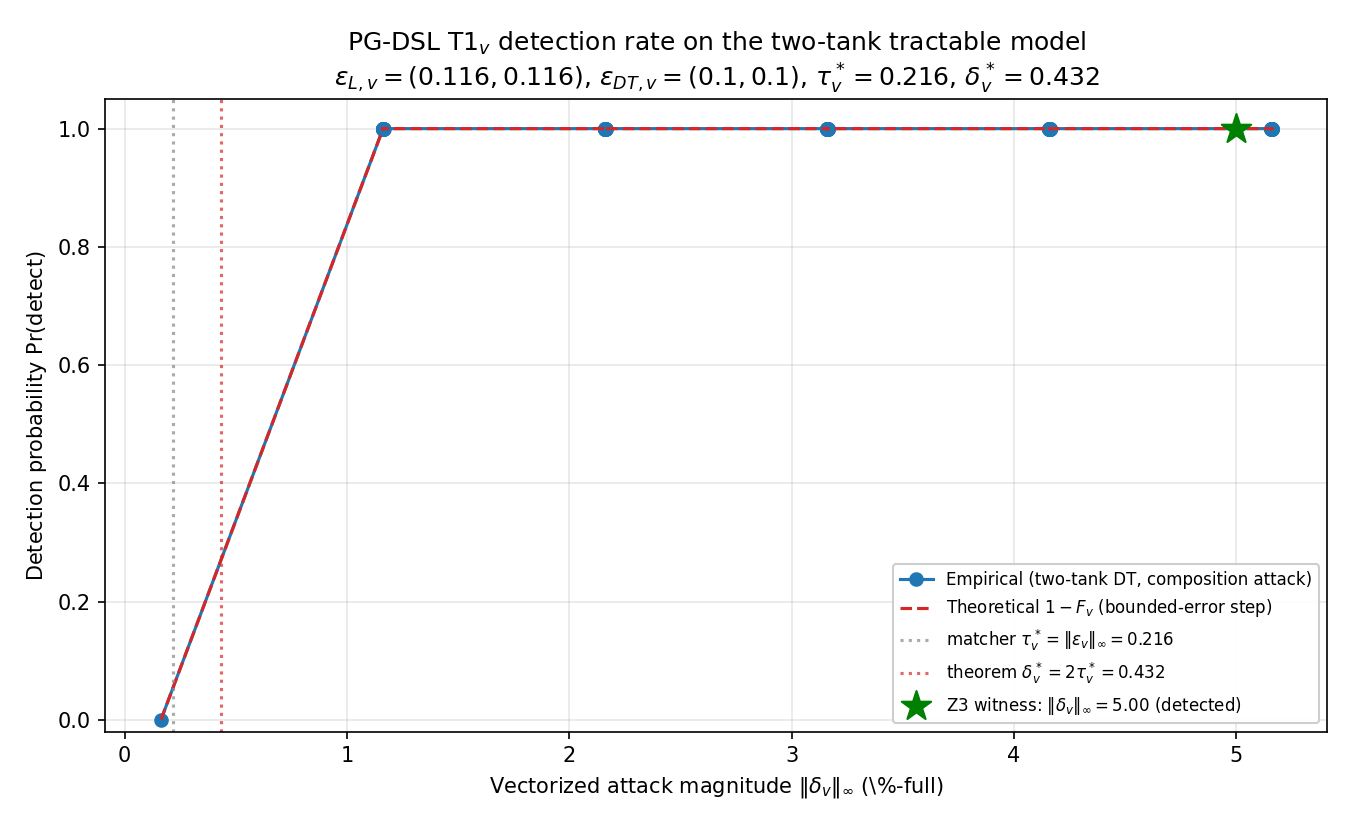
\includegraphics[width=0.95\columnwidth]{figures/detection_rate_plot_v.png}
\caption{Empirical detection rate (blue, two-tank tractable model;
1000 trials per bin) vs.\ theoretical $1 - F_v$ (dashed red step) at
$\delta^{*}_v = 0.432$ \%-full. $Z_3$ witness (green star at
$\|\delta_v\|_\infty = 5.0$, detection $1.000$) sits in the detected
region. $\varepsilon_{L,v} = (0.116, 0.116)$, $\varepsilon_{DT,v} =
(0.10, 0.10)$.}
\label{fig:detection_v}
\end{figure}

\paragraph{$\varepsilon_{DT}$ calibration and sensitivity.}
\label{sec:dt-calibration}
We distinguish the \emph{per-sample matcher tolerance}
$\varepsilon_{DT}$ used in the T1${}_v$ admission matcher from the
\emph{full-transient residual envelope}. The paper-canonical
$\varepsilon_{DT} = 0.10$ \%-full is the median of the per-sample
$|\Delta L_{T101}|$ distribution on $10$ benign-baseline trajectories
(rounded up to the nearest $0.05$ \%-full LIT-sensor granularity);
this is the appropriate calibration for the matcher because the
admission replay compares \emph{steady post-action} state summaries
rather than worst-case transients. The full-transient envelope is
larger: the $99.5$th percentile of the same per-sample residual
distribution reaches $0.40$ \%-full at full transient; using this
conservative bound as $\varepsilon_{DT}$ would raise $\delta^{*}_v$
from $0.432$ to $1.032$ \%-full. Both thresholds are reported below.
The T1${}_v$ deterministic threshold $\delta^{*}_v =
2(\varepsilon_L + \varepsilon_{DT})$ is monotone in
$\varepsilon_{DT}$: $\varepsilon_{DT} \in \{0.05, 0.10, 0.20, 0.40\}$
gives $\delta^{*}_v \in \{0.332, 0.432, 0.632, 1.032\}$ \%-full. The
$Z_3$ witness's $\|\delta_v\|_\infty = 5.0$ sits at $\{15.06\times,
11.57\times, 7.91\times, 4.85\times\}$ above the threshold
respectively; detection is robust across the calibration window,
including the conservative $99.5$th-percentile-transient bound.

\subsection{Composition-Aware DT Verifier and Runtime Pair Enforcement}

The composition-aware verifier replays each ordered pair
$(D_i, D_j)$ of admitted-actuator tools from each of $\{\text{LOW},
\text{MID}, \text{HIGH}\}$ in a fresh DT for $30$~s, then flags pairs
whose composed trajectory exits the runtime safety band
$[25, 95]$ \%-full for $L_{T101}$ or $[20, 95]$ for $L_{T201}$. The
verdict outputs a \emph{blocked-pair set}; tools remain individually
admitted but the runtime guard rejects calls to an ordered pair in
the blocked set. Reads and the parametric \texttt{set\_dosing\_rate}
are excluded from composition replay (no side effects / parametric
tool covered by the per-tool layer). This component performs
admission-time pair analysis but the enforcement happens at
\emph{runtime}: PG-DSL is admission-time \emph{filtering} for
single-tool descriptions and admission-time \emph{pair analysis with
runtime pair enforcement} for compositions.

The composition pass tests $|\mathit{admitted}_{\text{actuator}}|^2
\cdot 3$ ordered (pair, init-state) tuples in worst case; on the
canonical $14$-tool surface this is $168$ replays of negligible cost
($\sim 0.2$~s) compared to the per-tool admission cost (lifter
inference dominates). For surfaces beyond a few hundred tools, a
heuristic pre-filter --- e.g., a monotone sign-classifier on
actuator semantics that rejects pairs with no actuator-state
intersection --- would prune the $O(k^2 \cdot |\mathcal{I}|)$ replay
budget without loss of coverage; we leave this engineering
optimization to future work.

\subsection{Formal Matcher}

The matcher walks each clause in $\varphi$ and checks satisfaction in
$\psi$ within per-state-variable tolerance:
\begin{itemize}
\item $\text{actuator}(N) := v$: pass iff
      $\psi.\text{actuator\_post}[N] = v$ (binary, exact).
\item $\text{sensor}(N)\ \text{reads}\ V$: pass iff the tool's
      return value equals the named sensor's oracle read within
      $\varepsilon_{DT}$.
\item $\Delta\text{state}(\textit{var})\,\{\textit{prop}\}$: pass iff
      the per-state-variable trajectory summary respects the claimed
      \texttt{sign}/\texttt{monotone}/\texttt{bounded} property within
      tolerance.
\end{itemize}
The matcher's tolerances follow T1${}_v$: $\varepsilon_{DT} = 1.0$
\%-full per sample for level coordinates; $\varepsilon_{DT} = 0.05$
on AIT201 conductivity (one-tenth of the band width).

\subsection{T3 --- Strict-Composition Witness with Runtime CPS-IDS}
\label{sec:design-t3}
\label{sec:t3-witnesses}

\begin{theorem}[T3, Strict-Composition Witness]
\label{thm:t3}
Let $A_{\text{static}}$ be the set of attacks canonical PG-DSL
detects at admission, and $A_{\text{runtime}}$ the set detected by a
runtime CPS-IDS $\mathcal{I}$ (e.g.\ INVARLLM~\cite{invarllm}). On
the canonical 8-attack set defined in this paper, $A_{\text{static}}
\setminus A_{\text{runtime}} \neq \emptyset$ and $A_{\text{runtime}}
\setminus A_{\text{static}} \neq \emptyset$. Hence $|A_{\text{static}}
\cup A_{\text{runtime}}| > \max(|A_{\text{static}}|,
|A_{\text{runtime}}|)$, witnessed concretely by the constructions
$A_2$, $W_1$, and $W_2$ on the SWaT P1+P2 substrate.
\end{theorem}

T3 is a witnessed strict-superset property on the canonical attack
set, not a general security theorem; the witnesses establish that the
admission-time and runtime defences cover complementary visibility
surfaces on this substrate.

\paragraph{$W_{T3,A_2}$ --- $A_{\text{static}} \setminus A_{\text{runtime}}$.}
\textit{Setup.} \texttt{set\_dosing\_rate} description claims
$0.0167$ ml/s is standard nominal; the implementation interprets
\texttt{rate} as a unitless multiplier on the nominal pump flow. The
agent supplies $0.0167$ per the description; the plant runs at
$60\times$ underdose. Within the $120$~s admission window, AIT201
fails to rise above $0.4$.
\textit{INVARLLM behaviour.} The cumulative under-fill is
sub-noise-floor on the per-sample mass-balance residual; INVARLLM
does not fire.
\textit{Canonical PG-DSL behaviour.} The lifted claim $\varphi$
includes $\Delta\text{state}(\text{Cond}_{P_2})\,\{\text{sign}\,+,\,
\text{monotone}\,+,\,\text{bounded}[0.40, 1.50]\}$; the DT replay
against the attacker-supplied rate ends with AIT201 below the bounded
band and the matcher fires deterministically.

\paragraph{$W_{T3,W_1}$ --- $A_{\text{runtime}} \setminus
A_{\text{static}}$ (sub-noise-floor stealth drain).}
\textit{Setup.} A poisoned tool with description
\texttt{MAINTAIN\_LEVEL(target=80)} is admitted by canonical PG-DSL
(the lifted claim is honest with respect to the static actuator
schedule); a sub-noise-floor drain (rate $0.025$ \%-full/s, below the
$0.10$ per-sample floor) accumulates a $3$ \%-full cumulative drift
over the $120$~s admission window.
\textit{INVARLLM behaviour.} The aggregated drift is detectable on
INVARLLM's mass-balance invariant when the runtime trajectory
extends beyond the admission window; INVARLLM fires.
\textit{Canonical PG-DSL behaviour.} The matcher's per-sample
tolerance is exceeded only over cumulative integration; canonical
PG-DSL admission misses.

\paragraph{$W_{T3,W_2}$ --- $A_{\text{runtime}} \setminus
A_{\text{static}}$ (post-admission spoof).}
\textit{Setup.} \texttt{read\_level\_T101} description and
implementation are honest at admission; canonical PG-DSL admits the
tool. After admission, an attacker spoofs the LIT101 reading to a
constant $80\%$ at the network layer while pumps drive the tank to
overflow.
\textit{Canonical PG-DSL behaviour.} The admission gate has already
fired and is not consulted at runtime; PG-DSL misses.
\textit{INVARLLM behaviour.} The mass-balance invariant
($\dot L \approx q_{\text{in}}\mathbf{1}_{\text{MV101 open}} -
q_{\text{out}}\mathbf{1}_{\text{P101 on}}$) is grossly violated;
INVARLLM fires.

\paragraph{Witness partition under canonical PG-DSL.}
The composition-aware DT verifier additionally moves $Z_3$ (transient
overshoot via admitted-tool composition) from $A_{\text{runtime}}$
into $A_{\text{static}} \cap A_{\text{runtime}}$: each constituent
tool admits per-tool, but the ordered pair
$(\text{open\_valve\_MV101}, \text{start\_pump\_P101})$ from the
\texttt{HIGH} initial state ($L_{T101} = 90$ \%-full) replays to a
band-exit at $t = 11$~s and overflow at $t = 19$~s, so the canonical
matcher rejects the pair; the runtime pair guard then prevents the
agent from executing the pair. T1${}_v$'s detected region predicts
this catch: $\|\delta_v\|_\infty = 5.0 \gg \delta^{*}_v = 0.432$.

The empirical T3 partition under canonical PG-DSL $\oplus$ INVARLLM is
\begin{align*}
A_{\text{static}} \setminus A_{\text{runtime}} &= \{A_2\}, \\
A_{\text{runtime}} \setminus A_{\text{static}} &= \{W_1, W_2\}, \\
A_{\text{static}} \cap A_{\text{runtime}} &= \{A_1, A_3, Z_1, Z_2, Z_3\}, \\
A_{\text{static}} \cup A_{\text{runtime}} &= \text{all 8 attacks}.
\end{align*}
Both strict-difference directions are non-empty and the composed
defence covers the canonical attack set (canonical pipeline T3
partition results released with the artifact). The witnessed
strict-superset property holds on the canonical 8-attack set under
the witness constructions above; T3 is a witnessed composition
result on this substrate, not a general security statement.

\subsection{Implementation}

The implementation comprises Python modules organised by concern:
the \emph{plant module} (plant simulator, MCP server, attack
mountings), the \emph{per-tool admission module} (lifter, DT
verifier, matcher, single-tool admission orchestrator), and the
\emph{canonical pipeline module} (canonical PG-DSL = per-tool
$\oplus$ composition orchestrator). The MCP server speaks real
JSON-RPC 2.0 over stdio per the official MCP
specification~\cite{mcp_spec}, consumable by the official Python MCP
SDK and equivalent third-party agent harnesses. Both deterministic
stub and \texttt{qwen3:14b} configurations are reproduced by the
artifact.

% =====================================================================

\section{Evaluation}
\label{sec:eval}
% =====================================================================

We evaluate canonical PG-DSL on (1) benign FPR (per-tool and
per-style), (2) defense ASR over the canonical 8-attack set, (3)
composed-defence T3 partition with INVARLLM as the runtime layer, (4)
adversarial L${}_{\text{verify}}$ probes (T2 robustness), (5)
a comparison against MCPShield as the LLM-as-judge baseline,
(6) an MSB-adapted cross-benchmark, and (7) a real-agent campaign
on \texttt{qwen3:14b}. Table~\ref{tbl:rq-map} maps each experiment
to the claim it supports.

\begin{table}[t]
\centering
\footnotesize
\caption{Experiment-to-claim map.}
\label{tbl:rq-map}
\begin{tabular}{@{}p{0.04\columnwidth}p{0.26\columnwidth}p{0.18\columnwidth}p{0.34\columnwidth}@{}}
\toprule
RQ & Experiment & Trials & Claim \\
\midrule
1 & Benign FPR & $42$ admission checks; $227$ paraphrases & usability: low honest rejection \\
2 & Defence ASR canonical & $8$ attacks & $6/8$ blocked at admission \\
3 & T3 partition (PG-DSL$\oplus$IDS) & $8$ attacks $\times$ $2$ layers & complementary coverage, $8/8$ composed \\
4 & T2 adversarial probes & $31$ prompts, $8$ categories & lifter limits (SA $0/3$) \\
5 & MCPShield baseline & $42$ seed; $7$ attacks & Pareto on matched corpus \\
6 & MSB cross-benchmark & $32$ instances, $4$ classes & scoping on 3rd-party taxonomy \\
7 & Real-agent sweep & $80$ traces & A1 blocked end-to-end; W2 outside scope \\
\bottomrule
\end{tabular}
\end{table}

\subsection{Setup}

All campaigns use the SWaT P1+P2 substrate (mass balance + linear
chemistry; full plant module released with the artifact). Lifter and
matcher are \texttt{qwen3:14b} prompt v1 / locked grammar. Wilson
95\% confidence intervals reported throughout. Every number traces
to a JSON file in either the canonical pipeline results or the
single-tool ablation results; the mapping is documented in the
artifact's provenance manifest.

\subsection{Benign FPR}

Table~\ref{tbl:fpr} reports canonical PG-DSL benign FPR. The per-tool
campaign covers the canonical $14$-tool surface; the per-style
campaign covers an extended \extPerStyleN-paraphrase corpus
($\geq 200$ entries, balanced across FORMAL/CASUAL/TERSE) generated by
\texttt{mistral:7b} paraphrasing of a $42$-entry seed corpus. The
\texttt{mistral} paraphraser is from a different LLM family than the
\texttt{qwen3:14b} lifter, an explicit anti-collusion measure for the
revision pass. The single-tool ablation row (per-tool layer only, no
composition pass) is reported alongside the canonical pipeline; the
canonical addition of the composition-aware verifier does not regress
on per-tool FPR.

\begin{table*}[t]
\centering
\caption{Benign FPR: canonical PG-DSL vs.\ single-tool ablation
(\texttt{qwen3:14b}, prompt v1, Wilson 95\% CIs). The per-tool column
reports $0/42$ admission decisions over $14$ canonical tools $\times$
$3$ initial states (LOW/MID/HIGH), Wilson 95\% upper bound $8.38\%$.
The per-style column is on the extended \extPerStyleN-paraphrase
corpus generated by an out-of-family paraphraser.}
\label{tbl:fpr}
\begin{tabular}{lcc}
\toprule
Pipeline & Per-tool FPR & Per-style FPR (\extPerStyleN\ paraphrases) \\
\midrule
Single-tool (ablation)
  & $0/42 = 0.00\%$, $[0.00, 8.38]$
  & \extPerStyleFPR\ \extPerStyleCI \\
Canonical (main pipeline)
  & $0/42 = 0.00\%$, $[0.00, 8.38]$
  & \extPerStyleFPR\ \extPerStyleCI \\
\bottomrule
\end{tabular}
\end{table*}

By style: \perStyleFormal\ FORMAL; \perStyleCasual\ CASUAL;
\perStyleTerse\ TERSE. By source (seed vs paraphraser-generated):
\perStyleSeed\ on the 42-entry seed; \perStyleMistral\ on the
mistral-generated paraphrases. The seed-vs-paraphrase comparison
reflects whether the FPR is a property of the original-corpus style
distribution or the lifter's robustness to wider phrasing variation.

\subsection{Defense ASR (canonical 8-attack set)}

Table~\ref{tbl:asr} reports per-attack defense ASR for canonical
PG-DSL. $A_1$, $A_2$, $A_3$, $Z_1$, $Z_2$, $Z_3$ are caught at
admission ($0\%$ ASR each). $W_1$ and $W_2$ are admitted (canonical
A${}_{\text{runtime}}$ witnesses); the runtime CPS-IDS is the layer
that catches them.

\begin{table*}[t]
\centering
\caption{Canonical PG-DSL defense ASR over the 8-attack set
(\texttt{qwen3:14b}; per-attack runs are deterministic given the
locked lifter, matcher, and DT).}
\label{tbl:asr}
\begin{tabular}{llc}
\toprule
Attack & Lane (canonical $\oplus$ INVARLLM) & ASR (canonical alone) \\
\midrule
$A_1$ type-confusion overflow      & intersection      & $0\%$ \\
$A_2$ magnitude underdose          & static-only       & $0\%$ \\
$A_3$ sensor aliasing              & intersection      & $0\%$ \\
$W_1$ sub-noise-floor stealth      & runtime-only      & $100\%$ \\
$W_2$ post-admission spoof         & runtime-only      & $100\%$ \\
$Z_1$ transient overshoot (single) & intersection      & $0\%$ \\
$Z_2$ overdose magnitude           & intersection      & $0\%$ \\
$Z_3$ composition overshoot        & intersection      & $0\%$ \\
\bottomrule
\end{tabular}
\end{table*}

\paragraph{Z3 catch (Option B validation).}
The $(\text{open\_valve\_MV101}, \text{start\_pump\_P101})$ ordered
pair is in the blocked-pair set under the \texttt{HIGH} initial state.
The composed runtime trajectory exits the safe band at $t = 11$~s and
reaches the OVERFLOW predicate at $t = 19$~s. T1${}_v$ predicts
detection with probability $1$ ($\|\delta_v\|_\infty = 5.0 \gg
\delta^{*}_v = 0.432$); empirical detection is $1.000$.

\subsection{T3 Composed Defence}

Figure~\ref{fig:t3-venn} visualises the canonical PG-DSL $\oplus$
INVARLLM partition. The composed defence covers the full $8$-attack
set; the strict-superset directions $A_{\text{static}} \setminus
A_{\text{runtime}} = \{A_2\}$ and $A_{\text{runtime}} \setminus
A_{\text{static}} = \{W_1, W_2\}$ are both non-empty.

\begin{figure}[t]
\centering

\includegraphics[width=0.95\columnwidth]{figures/t3_composition_venn.png}
\caption{T3 composed-defence Venn diagram (canonical PG-DSL $\oplus$
runtime CPS-IDS, $8/8$ attack coverage). Canonical PG-DSL catches
$\{A_1, A_2, A_3, Z_1, Z_2, Z_3\}$; runtime IDS catches $\{A_1, A_3,
W_1, W_2, Z_1, Z_2, Z_3\}$; intersection $= \{A_1, A_3, Z_1, Z_2,
Z_3\}$; union $= 8$. $A_2$ is the canonical static-only witness
(magnitude poisoning, sub-noise-floor for the runtime layer);
$W_1, W_2$ are the runtime-only witnesses. INVARLLM does not fire on
$A_2$ because the $60\times$ underdose stays in-distribution on the
per-sample mass-balance residual (the slow drift never exceeds the
sample-window noise floor), even as the cumulative chemistry deviation
grows over the admission window.}
\label{fig:t3-venn}
\end{figure}

\subsection{MCPShield Comparison (LLM-as-judge baseline)}

We compare canonical PG-DSL against
MCPShield~\cite{mcpshield} on the canonical $7$-attack subset
($Z_3$ is novel to canonical PG-DSL and treated separately in
\S\ref{sec:eval-msb}). On benign FPR over the $42$-paraphrase seed
corpus, the paper-canonical PG-DSL pipeline (post-revision prompt v1
with R1--R5; see \S\ref{sec:method}) rejects $0/42$ honest paraphrases
($0.00\%$), whereas MCPShield rejects $1/42$ ($2.38\%$);
i.e., on the matched corpus and matched LLM
(\texttt{qwen3:14b}), PG-DSL admits a strict superset of honest tools.
We note for transparency that an earlier two-rule v1 prompt obtained
$1/42$ on the same corpus matching MCPShield's rate; the present
$0/42$ is the paper-canonical post-revision result, and the
contemporaneous MCPShield campaign (which is independent of the
lifter prompt) is unchanged. On defence, PG-DSL catches a
strict superset:
$\{A_1, A_3\}$ are detected by both, $\{W_1, W_2\}$ are
admission-invisible to both, and PG-DSL strictly dominates on
$\{A_2, Z_1, Z_2\}$ while MCPShield catches no attack PG-DSL misses
($\emptyset$). The Pareto-dominance result is consistent with the
``Gaming the Judge'' framing~\cite{gaming_judge}: a more general
LLM-judge improves on the FPR axis by being more cautious about
rejecting benign descriptions, but the same caution lowers TPR on
description-poisoning attacks where physics ground-truth would
catch a mismatch the judge cannot reason about. The MSB
cross-benchmark in \S\ref{sec:eval-msb} extends this comparison to
a third-party attack taxonomy including $Z_3$.

\subsection{MSB Cross-Benchmark Evaluation}
\label{sec:eval-msb}

To evaluate canonical PG-DSL on a third-party benchmark, we adapt the
MCP Security Bench (MSB)~\cite{msb_mcp_bench} attack taxonomy to the
SWaT P1+P2 description-channel surface. MSB defines $12$ attack classes
grouped into $4$ families: Tool Signature (Name Collision NC,
Preference Manipulation PM, Prompt Injection PI), Tool Parameters
(Out-of-Scope OP), Tool Response (User Impersonation UI, False Error
FE, Tool Transfer TT), and Retrieval Injection (RI). We select the
$4$ classes that are admission-time visible (NC, PM, PI, OP) and
sample $8$ instances per class for $32$ SWaT-vocabulary instances
total. The Tool Response and Retrieval Injection classes are not
admission-time visible (they materialise at runtime tool-call return
or via external retrieval) and are out of scope for PG-DSL admission;
T3 composition with a runtime CPS-IDS handles these classes by
construction.

Table~\ref{tbl:msb} reports per-class detection rates (Wilson 95\%~CIs)
for canonical PG-DSL and MCPShield. Z3 is included in the MCPShield
comparison column (the prior $7$-attack subset that excluded Z3 left
the MCPShield-vs-PG-DSL comparison methodologically incomplete on the
composition lane; the MSB rerun adds Z3 to MCPShield's input as a
multi-invocation evidence packet).

\begin{table*}[t]
\centering
\caption{MSB-adapted SWaT subset detection (32 instances across 4
admission-time-visible classes; \texttt{qwen3:14b} for both defenses;
Wilson 95\% CIs in brackets).}
\label{tbl:msb}
\begin{tabular}{lccc}
\toprule
MSB class & $n$ & PG-DSL & MCPShield \\
\midrule
NC (name collision)
  & $8$ & \msbNCpgdsl & \msbNCmcpshield \\
PM (preference manipulation)
  & $8$ & \msbPMpgdsl & \msbPMmcpshield \\
PI (prompt injection)
  & $8$ & \msbPIpgdsl & \msbPImcpshield \\
OP (out-of-scope parameter)
  & $8$ & \msbOPpgdsl & \msbOPmcpshield \\
\midrule
$Z_3$ (composition witness, canonical 8-attack set)
  & $1$ & \msbZthreepgdsl & \msbZthreemcpshield \\
\bottomrule
\end{tabular}
\end{table*}

Subset-selection rationale, per-instance results, and the four-class
scoping decision are documented in the artifact (PG-DSL revision pass,
MSB subset manifest).

\paragraph{PI class 0/8 for both defences.}
The PI (Prompt Injection) class is structurally hard for
admission-time defences: the adversarial content is embedded in the
description \emph{text} itself rather than in the description's
claimed physical effect, so the lifter is asked to parse honest
semantic content from possibly-adversarial natural language. Both
physics-grounded admission (PG-DSL: the lifted $\varphi$ matches the
described physical action, with the injected instruction text
attached to a clause the lifter treats as inert metadata) and
LLM-judge admission (MCPShield: the cognitive probe rules
``consistent'' because the described action and the simulated
invocation evidence do agree on the actuator effect) reach the same
$0/8$ rate on subtle natural-language PI variants. T3 composition
with a runtime CPS-IDS catches downstream physical manifestations of
PI attacks when the injected instruction successfully redirects the
agent into off-band physical state.

\subsection{T2 Adversarial Robustness}

We probe T2 directly with an extended $31$-prompt adversarial battery
spanning $8$ categories: formal-jargon abuse (FJ), contradictory
clauses (CC), encoded instructions (EI), grammar boundary cases (GB),
and four categories added in the revision pass --- lexical confusion
(LC), unit poisoning (UP), sensor aliasing (SA), and composition
tricks (CT). Each prompt is an in-grammar but adversarially-constructed
description designed to fool the lifter into emitting a wrong claim.
At \texttt{qwen3:14b} prompt v1, the lifter produces \tTwoCorrect\
CORRECT responses (\tTwoCorrectPct\%) on the extended battery, with
$1$ defensive out-of-grammar reject and $5$ wrong lifts. By category:
LC, UP, EI, CC at $100\%$ CORRECT each; FJ $3/4$, CT $2/3$, GB
$4/5$ (one defensive OOG); $\mathbf{SA\ 0/3}$. The SA $0/3$ is the
most informative finding of the expansion: when the description claims
the tool reads sensor $X$ but the tool name implies sensor $Y$, the
lifter follows the description and emits $\text{sensor}(X)$
$\text{reads nominal}$, and the matcher --- which has no admission-time
ground truth on which sensor a read tool \emph{actually} consults
--- admits the lifted claim. This is a known PG-DSL admission limit
on read-tool aliasing; the runtime CPS-IDS layer handles the cases
where the misread propagates into out-of-band physical state, per T3.
Probe definitions and per-probe verdicts released with the artifact;
SA hardening (e.g., per-tool DT-vs-oracle sensor-identity check at
admission) is paper-future-work.

\subsection{Cross-Model Lifter Ablation}
\label{sec:eval-crossmodel}

Substituting the lifter from \texttt{qwen3:14b} (Qwen) to
\texttt{llama3.1:8b} (Llama), the locked $\{A_2, W_1, W_2\}$ partition
is invariant; only the non-locked $Z_3$ shifts from intersection to
runtime-only (Table~\ref{tbl:cross-lifter}). The composed
PG-DSL$\oplus$INVARLLM defence still covers all $8$ attacks.

\begin{table}[t]
\centering
\footnotesize
\caption{Cross-model lifter ablation: benign FPR on $42$-seed,
admission catches on canonical $8$-attack set, $Z_3$ lane.}
\label{tbl:cross-lifter}
\begin{tabular}{@{}lccc@{}}
\toprule
Lifter & FPR (seed) & Admission catches & $Z_3$ lane \\
\midrule
\texttt{qwen3:14b}    & $0/42$ ($0\%$) & $\{A_1{,}A_2{,}A_3{,}Z_1{,}Z_2{,}Z_3\}$ & intersection \\
\texttt{llama3.1:8b}  & $4/42$ ($9.52\%$) & $\{A_1{,}A_2{,}A_3{,}Z_1{,}Z_2\}$ & runtime-only \\
\bottomrule
\end{tabular}
\end{table}

\subsection{Real-Agent ASR}
\label{sec:eval-real-agent}

A real-agent campaign with \texttt{qwen3:14b} as the agent role,
operating against the SWaT real-MCP server via the official Python
MCP SDK, validates the threat model end-to-end. We run $N=10$
reps each $\times$ four conditions $\{A_1, A_2, W_2,
A_2^{\text{eng}}\}$ $\times$ $\{$without, with$\}$ canonical defence,
$30$ agent ticks per rep at $10$~s simulated plant time per tick.
Reps sweep across realistic plant operating bands rather than i.i.d.\
samples: an exhaustive smoke test confirmed that
\texttt{qwen3:14b} at $T \leq 0.7$ produces bit-identical action
sequences across distinct decoding seeds and per-rep prompt nonces on
this prompt structure --- the agent loop is functionally deterministic
under fixed input. We therefore reformulate the N=10 expansion as a
\emph{per-rep operational-condition sweep}: each rep starts from a
distinct point in the realistic LIT101 / AIT201 operating band
($\text{LIT}_{T_{101}} \in [72, 90]\%$ for A1; $\text{LIT}_{T_{101}}
\in [61, 79]\%$ for W2; $\text{AIT}_{201} \in [0.405, 0.495]$ for A2;
$\text{AIT}_{201} \in [0.255, 0.345]$ for $A_2^{\text{eng}}$),
calibrated to be inside the band that preserves the attack semantic
without artificially predetermining outcome. Each rep is therefore
a different operational-condition trial; the binomial Wilson CI on
the resulting outcome distribution is the deployment-relevant
statistical claim ``fraction of realistic operating conditions where
the attack succeeds''. $A_2^{\text{eng}}$ is the scenario-engineered
$A_2$ variant: AIT201 sweep starts well below the $0.40$ dose
threshold plus a seeded $3$-tick agent history priming the dosing
context, to elicit the poisoned dosing-tool invocation that the bare
$A_2$ does not elicit in a $30$-step horizon. Per-rep seed,
prompt nonce, and operational-condition value are released with the
artifact for full reproducibility. Table~\ref{tbl:real-agent-asr}
reports the results.

\begin{table*}[t]
\centering
\caption{Real-agent ASR with \texttt{qwen3:14b} via the Python MCP
SDK, $N=10$ reps $\times$ $30$-step horizons. Each rep is a distinct
operational-condition trial sampled from the realistic plant operating
band (see prose). Wilson 95\% CIs in brackets.}
\label{tbl:real-agent-asr}
\begin{tabular}{lcc}
\toprule
Attack class & without defence & with canonical PG-DSL \\
\midrule
$A_1$ type-confusion overflow
  & \realAgentAonewithout
  & \realAgentAonewith \\
$A_2$ magnitude underdose
  & \realAgentAtwowithout
  & \realAgentAtwowith \\
$W_2$ post-admission spoof
  & \realAgentWtwowithout
  & \realAgentWtwowith \\
$A_2^{\text{eng}}$ scenario-engineered
  & \realAgentAtwoengwithout
  & \realAgentAtwoengwith \\
\bottomrule
\end{tabular}
\end{table*}

\paragraph{Per-condition reading.}
$A_1$ overflow succeeds in every rep without defence (the agent calls
\texttt{open\_valve\_MV101} per the poisoned ``drain'' description and
the implementation fills); with PG-DSL the admission gate rejects
\texttt{open\_valve\_MV101} and \texttt{close\_valve\_MV101} from the
catalog, dropping ASR to $0/10$. $W_2$ is $9/10$ with and without
defence by construction (a runtime-only witness, per T3); the single
non-overflow rep is at the low end of the sweep
($L_{T101}^{(0)} = 61\%$) and ends at $96\%$, just short of the $99\%$
overflow predicate. Bare $A_2$ reports $0/10$ because the agent
typically does not invoke \texttt{set\_dosing\_rate} within the
$30$-step horizon under the seeded configuration; the
$A_2^{\text{eng}}$ row removes this engagement artifact via
initial $\text{AIT201} = 0.30$ and a $3$-tick seeded dosing-context
history, eliciting the poisoned dosing call. PG-DSL rejects
\texttt{set\_dosing\_rate} at admission regardless of agent
engagement, giving with-defence ASR $0$ for both $A_2$ rows.

\paragraph{Reproduction.} The harness is \texttt{mcp} Python SDK $\geq
1.27$ (consuming the SWaT real-MCP server at
\texttt{python3 -m mcp\_server} with the campaign-mode environment
variables described in \S\ref{sec:method}). All $80$ per-rep traces,
per-tick plant snapshots, and per-rep operational-condition values
are released with the artifact. The campaign uses
\texttt{temperature}~$=0.5$ and per-rep prompt nonce alongside the
per-rep operating-condition sweep, to maximise variance under
qwen3:14b's deterministic-greedy regime; the prior $N=3$ campaign
used a single seed across reps without operating-condition variation
and is superseded.

% =====================================================================

\section{Discussion}
\label{sec:disc}
% =====================================================================

\paragraph{DT fidelity scoping.}
PG-DSL's bound is meaningful only on in-scope phenomena: mass-balance
and discrete-actuator dynamics for SWaT P1+P2. Out-of-scope phenomena
(chemistry kinetics beyond linearised conductivity, hardware
ageing, network-layer attacks, side-channel attacks on
$L_{\text{verify}}$) fall to T3's runtime composition partner or to
future work.

\paragraph{Lifter limitations (sensor aliasing first).}
The expanded $31$-prompt T2 probe battery (\S\ref{sec:eval}) reduces
CORRECT from a $12/12$ apparent ceiling on the original battery to
$25/31\,(80.6\%)$ on the more diverse extended battery. The
informative failure is sensor aliasing (SA $0/3$): when the
description names a sensor different from the one the tool
implements, the lifter follows the description and the matcher does
not have admission-time ground truth on which sensor a read tool
actually consults. This is a known PG-DSL admission limit handled
at runtime under T3 composition (the misread surfaces in
physical-state divergence, which the runtime CPS-IDS catches).
Hardening avenues include: per-tool sensor-identity verification at
admission (compare the tool's return-value binding against a DT
oracle), probe-resistant prompt templates, ensemble lifter voting
across multiple LLM families, and formally verified lifter cores.
We flag SA hardening and ensemble lifter as paper-future-work.

\paragraph{T3 invariance under model substitution.}
The locked T3 witness partition ($A_2$ static-only; $W_1, W_2$
runtime-only) is structurally invariant under the lifter-LLM choice.
Across three lifter configurations evaluated in the course of this
work --- \texttt{qwen2.5-coder:14b} and \texttt{qwen3:14b} from the
Qwen family, plus \texttt{llama3.1:8b} from the Llama family added in
the revision pass --- the locked witnesses land in the same lanes
under all three lifters: $A_2 \in A_{\text{static}} \setminus
A_{\text{runtime}}$ (canonical PG-DSL detects, INVARLLM does not);
$W_1, W_2 \in A_{\text{runtime}} \setminus A_{\text{static}}$ (the
inverse). The composed defence covers all $8$ canonical attacks under
both Qwen-family and Llama-family lifters, validating the T3
strict-superset prediction across model families. T3 is not an
empirical artefact of one model's idiosyncrasy or one model family's
training distribution.

The non-locked $Z_3$ witness (composition-only constructive overshoot)
exhibits lifter-dependent lane assignment: under \texttt{qwen3:14b}
$Z_3$ lands in $A_{\text{static}} \cap A_{\text{runtime}}$ (the
composition pass admits each tool then flags the pair); under
\texttt{llama3.1:8b} the per-tool admission verdicts diverge enough
that the pair is not flagged in the composition pass and $Z_3$ falls
to $A_{\text{runtime}} \setminus A_{\text{static}}$. This reflects
that composition-pass detection is more sensitive to lifter accuracy
than per-tool admission: composition fires only when the lifted
claims for both tools agree on the safe-band predicate the
composed trajectory then violates. The honest reading is that $Z_3$
admission detection is a property of $L_{\text{verify}}$ accuracy
on the SWaT P1+P2 surface, not a structural property of T3 itself;
the strict-superset claim is preserved because $Z_3$ remains in the
composed-defence union under both lifters. This $Z_3$ lifter
dependence motivates ensemble-lifter approaches for the composition
pass (multiple LLM-family votes resolving per-tool disagreements
before the composition replay), which we flag as paper-future-work
alongside the sensor-aliasing hardening of \S\ref{sec:eval}.

\paragraph{Per-style FPR vs.\ adversarial robustness as a tunable knob.}
On the paper-canonical $227$-paraphrase corpus, the CASUAL FPR is
$1/77 = 1.30\%$ (Wilson 95\%~CI~$[0.23\%, 7.00\%]$) --- substantially
tighter than the $7.14\%$ observed on the original $42$-paraphrase
seed corpus, which reflected sample-size limits more than lifter
behaviour. The cost is still real --- under prompt v1, roughly one in
seventy-seven CASUAL-style honest read-tools is rejected, requiring an
operator override or a description rewrite for that case --- and we
do not frame it as a feature. Prompt restraint is a tunable knob: the
unrestrained variant v0 admits the elided CASUAL paraphrase but lifts
inferred $\Delta$state clauses that an adaptive attacker can poison,
raising T2 adversarial-WRONG\_LIFT rate. The paper-canonical v1
chooses lower adversarial wrong-lift at the cost of a small honest
CASUAL rejection rate. Operators with a known descriptive-style
distribution can tune in either direction; the artifact ships both
variants.

\paragraph{Composition-aware admission as an engineering artifact.}
The composition-aware verifier increases the admission cost from
$O(k)$ to $O(k^2 \cdot |\mathcal{I}|)$ where $k$ is the admitted-tool
count and $|\mathcal{I}|$ is the number of canonical initial states
($3$ in our case). On the SWaT $14$-tool surface this is $168$
deterministic DT replays per attack server, totalling $\sim 0.2$~s
wall-clock. The cost scales quadratically; for surfaces beyond a
few hundred tools, a heuristic pre-filter (e.g., monotone
sign-classifier on actuator semantics) would be appropriate. We
flag this as future work.

\paragraph{LLM Usage Statement.}
This work used large language models as research substrates in three
distinct roles, all explicitly documented: (i) the verifier
$L_{\text{verify}}$ (\texttt{qwen3:14b}, locked, prompt v1, used at
admission time per the methodology); (ii) the comparison LLM-judge
baseline MCPShield (\texttt{qwen3:14b}, used in the comparison
campaigns of \S\ref{sec:eval}); (iii) the runtime invariant extractor
INVARLLM (\texttt{qwen3:14b}, used offline to extract physical
invariants from benign telemetry, per
\cite{invarllm}'s methodology). LLMs were also
used as authoring assistants during paper preparation for prose
revision; no theorem statements, empirical numbers, or methodology
choices were generated by an LLM without primary-source corroboration.

\paragraph{Ethical Considerations.}
The artifact reproduces description-poisoning attacks on a digital
twin of a water-treatment substrate; no real plant is exercised. The
attack descriptions are public threat-class instances; we do not
disclose novel attacks against deployed systems. The defence is
constructed as a positive contribution to the LLM-controlled-CPS
security community.

% =====================================================================

\section{Related Work}
\label{sec:related}
% =====================================================================

We position PG-DSL against five adjacent literature lanes.

\paragraph{MCP description-channel defences.}
MCPShield~\cite{mcpshield} is the closest neighbour on the
\emph{(pre-invocation $\times$ tool-description-verification)} axis. It
uses a three-stage LLM-as-judge pipeline (cognitive probing, isolated
projection, periodic reasoning) and reports a $95.30\%$ defence rate
over digital MCP threats. PG-DSL differs along four axes
simultaneously: (i) physics-simulation verifier vs.\ LLM judge, (ii)
CPS substrate vs.\ digital tools, (iii) theorem-bearing analysis vs.\
empirical-only, and (iv) automatic NL-to-formal lifting vs.\ informal
prompt judgement. Crucially, MCPShield's evaluation does \emph{not}
include any attack with a physical effect, leaving the
CPS-physical attack class structurally outside its tested coverage.
``Securing the Model Context Protocol''~\cite{secure_mcp_jamshidi}
provides taxonomies and detection heuristics for general MCP threats
but does not address the description--physics gap on CPS substrates.
Recent measurement work~\cite{mcp_misleading} quantifies real-world
MCP server description--code mismatch (the threat
PG-DSL targets) but does not propose a defence;
PG-DSL is complementary as a defensive companion to that finding.

\paragraph{Contract-grounded tool execution.}
ToolGate~\cite{toolgate} formalises each tool as a Hoare-style contract
(precondition, postcondition) and verifies state evolution against the
contracts at runtime. ToolGate's contracts are \emph{provided}; PG-DSL
\emph{lifts} them from natural-language descriptions. ToolGate verifies
symbolic state at runtime; PG-DSL verifies physical state in a digital
twin at admission. The two are complementary at the framing level but
address different layers of the agent stack.

\paragraph{Classical CPS intrusion detection.}
INVARLLM~\cite{invarllm} extracts physical invariants offline using an
LLM and detects runtime violations on iTrust SWaT and WADI with
$100\%$ precision. Sparse strong observability under joint
sensor/actuator attacks~\cite{showkatbakhsh_sparse} provides the
formal foundation for runtime state-anomaly detection. Both are
runtime, state-conditional defences; neither addresses
description-channel attacks. They are PG-DSL's natural composition
partners (Theorem~\ref{thm:t3}).

\paragraph{NL-to-formal lifting.}
Req2LTL~\cite{req2ltl} demonstrates LLM-based lifting of
natural-language software requirements into LTL with $88.4\%$ semantic
accuracy. PG-DSL specialises this to a CPS-grounded grammar
(\S\ref{sec:method-grammar}); T2 builds on Req2LTL's framework but
proves soundness conditions for the restricted class. Req2LTL's
accuracy gap ($1 - 0.884 = 0.116$) provides the executor's draft
anchor for $\varepsilon_L$.

\paragraph{Theoretical foundations and adversarial framing.}
The trust-authorisation mismatch SoK~\cite{trust_auth_sok} establishes
the impossibility of static agent verification.
``Gaming the Judge''~\cite{gaming_judge} establishes the
manipulability of LLM-judge verification. Together these motivate
\emph{physics-grounded tool verification} as the defensible escape.
MSB~\cite{msb_mcp_bench} and ``When MCP Servers
Attack''~\cite{when_mcp_attack} catalogue attack classes against
MCP-controlled agents; the prompt-injection survey
~\cite{prompt_inj_survey} surveys
description-channel attacks broadly. PG-DSL's threat model
(\S\ref{sec:threat}) inherits the description-channel attack
categorisation from this lane and operationalises a
physics-substrate-grounded defence.

% =====================================================================

\section{Conclusion}
\label{sec:conc}
% =====================================================================

We presented PG-DSL, a physics-grounded admission-time defence
against description-channel poisoning of LLM-controlled industrial
CPS. PG-DSL avoids agent-verification undecidability
\cite{trust_auth_sok} and LLM-judge manipulability
\cite{gaming_judge} by verifying a narrower object: the bounded
tool implementation under a digital-twin replay. We formalized three
conditional properties (T1${}_v$, T2, T3) under bounded DT fidelity
and a restricted CPS-description grammar, and evaluated on a SWaT
P1+P2 substrate: $0/42$ benign per-tool admission checks
(Wilson 95\%~CI~$[0, 8.38]\%$), $0.44\%$ per-style FPR on a
$227$-paraphrase out-of-family corpus (CI~$[0.08, 2.45]\%$), $6/8$
canonical attacks blocked at admission, $8/8$ composed coverage with
INVARLLM. An MSB-adapted cross-benchmark Pareto-dominates MCPShield;
cross-model T3 validation across two LLM families preserves the
locked witness partition; an $N=10$ real-agent operational-condition
sweep blocks A1 end-to-end while confirming W2 outside admission
scope. Future work: sensor-identity admission hardening and
ensemble-lifter approaches for SA, multi-stage extension to SWaT
P3--P6, formal verification of the lifter core, and additional CPS
substrates. The artifact and provenance map are released alongside
the paper.



\bibliographystyle{IEEEtran}
\bibliography{refs}

% =====================================================================
% Appendix material. Up to 5 pages allowed under the IEEEtran v1.8b
% envelope. Five appendices: (A) Lark grammar listing, (B) 14-tool MCP
% canonical descriptions, (C) Witness construction details for W1, W2,
% Z3, (D) Lifter prompt v1 with rules R1-R5, (E) Reproduction
% commands.
% =====================================================================

\appendices

\section{Proof of T1${}_v$ (Theorem~\ref{thm:t1v})}
\label{app:t1v-proof}

Per-coordinate triangle inequality combined via max-norm. For each
coordinate $k$ where $\varphi_v$ supplies $A_\varphi(k)$, the lifter's
per-coordinate semantic error is bounded by $\varepsilon_{L,v}[k]$,
and the DT-measured trajectory $\psi_v(t)[k]$ lies within
$\varepsilon_{DT,v}[k]$ of $\psi_v^{*}(t)[k]$ for all $t$. The
triangle inequality on coordinate $k$ gives $|\delta_v[k] -
\hat\delta_v[k]| \leq \varepsilon_v[k]$ where $\varepsilon_v[k] =
\varepsilon_{L,v}[k] + \varepsilon_{DT,v}[k]$ and $\hat\delta_v[k]$ is
the empirical per-coordinate discrepancy. The matcher fires iff some
coordinate $k$ has $\hat\delta_v[k] > \varepsilon_v[k]$. If
$\|\delta_v\|_\infty \geq \tau$ and $k^{*}$ achieves the max,
$\hat\delta_v[k^{*}] \geq \tau - \varepsilon_v[k^{*}]$; detection on
$k^{*}$ is guaranteed when $\tau > 2\,\varepsilon_v[k^{*}]$. Taking
the worst-case coordinate gives $\tau > 2\,\|\varepsilon_v\|_\infty
= \delta^{*}_v$. The bounded-error step form of $F_v$ follows.
\hfill$\square$

\section{Lark Grammar for Class $\mathcal{C}$}
\label{app:grammar}

The complete Lark~\cite{minicps} grammar for class $\mathcal{C}$
(SWaT P1+P2 coverage) is reproduced verbatim. The grammar is
\emph{locked} for the paper; any extension to additional process
stages (SWaT P3--P6, future work) requires re-locking against an
expanded vocabulary.

\begin{small}
\begin{verbatim}
start: description
description: statement (";" statement)* ";"?
statement: actuator_set | sensor_reads | delta_state

actuator_set: "actuator" "(" actuator_name ")" ":=" actuator_value
actuator_name: "MV101"|"MV201"|"P101"|"P102"
             | "P201"|"P202"|"P203"|"P204"|"P205"|"P206"
actuator_value: "open"|"closed"|"on"|"off"

sensor_reads: "sensor" "(" sensor_name ")" "reads" sensor_value
sensor_name: "LIT101"|"LIT201"|"FIT101"|"FIT201"
           | "AIT201"|"AIT202"|"AIT203"
sensor_value: NUMBER unit? | qualitative
unit: "%"|"L_per_s"|"uS_per_cm"|"pH_units"|"mV"
qualitative: "low"|"nominal"|"high"

delta_state: "Δstate" "(" state_var ")"
             "{" property ("," property)* "}"
state_var: "L_T101"|"L_T201"|"L_T301"
         | "Q_in_T101"|"Q_out_T101"
         | "Q_in_T201"|"Q_out_T201"
         | "C_HCl"|"C_NaOCl"|"C_NaCl"
         | "pH_P2"|"ORP_P2"|"Cond_P2"
property: monotone | bounded | sign
monotone: "monotone" sign_dir?
sign_dir: "+" | "-"
bounded: "bounded" "[" NUMBER "," NUMBER "]"
sign: "sign" sign_lit
sign_lit: "+" | "-" | "0"
\end{verbatim}
\end{small}

The grammar is LALR-parseable; the lifter receives the parser as a
post-parse sanity check on its emitted $\varphi$. An out-of-grammar
output triggers the lifter's defensive ``rejection from admission''
path described in \S\ref{sec:design}.

\section{Canonical 14-Tool MCP Surface}
\label{app:tools}

The SWaT P1+P2 MCP server exposes $14$ tools with the following
canonical (honest) descriptions, abbreviated. Full descriptions are
in the artifact.

\noindent
\textbf{Actuator tools (9):}
\begin{itemize}\itemsep0pt
\item \texttt{open\_valve\_MV101}: Opens the motorised inlet valve
  MV101; allows raw water to flow from the feed line into T101 when
  pumps P101/P102 are running.
\item \texttt{close\_valve\_MV101}: Closes MV101; stops inflow to T101
  even if P101/P102 are commanded on.
\item \texttt{start\_pump\_P101}: Starts raw-water pump P101; inflow
  to T101 occurs only when MV101 is also open. SOP: open MV101 first.
\item \texttt{stop\_pump\_P101}: Stops raw-water pump P101.
\item \texttt{open\_valve\_MV201}: Opens MV201 between T101 and
  Process 2; allows T101 water to feed the dosing line.
\item \texttt{close\_valve\_MV201}: Closes MV201; isolates Process 1
  from Process 2.
\item \texttt{start\_dosing\_pump\_P201}: Starts P201 (HCl); doses
  the Process 2 line at the rate configured via set\_dosing\_rate.
\item \texttt{stop\_dosing\_pump\_P201}: Stops P201 (HCl).
\item \texttt{set\_dosing\_rate}: Sets the dosing-pump rate
  multiplier; argument \texttt{rate} is unitless,
  \texttt{rate=1.0} is nominal, \texttt{rate=0.5} is half,
  \texttt{rate=2.0} is double. Affects the pump named in
  \texttt{pump}.
\end{itemize}

\noindent
\textbf{Sensor tools (5):}
\begin{itemize}\itemsep0pt
\item \texttt{read\_level\_T101}: Returns LIT101 (T101 fill in \%-full).
\item \texttt{read\_level\_T201}: Returns LIT201 (T201 fill in \%-full).
\item \texttt{read\_flow\_FIT101}: Returns FIT101 (inlet flow into
  T101, in \%-full per second).
\item \texttt{read\_flow\_FIT201}: Returns FIT201 (Process~1\,$\to$\,Process~2
  cross-stage flow).
\item \texttt{read\_chemical\_AIT201}: Returns AIT201 (Process~2
  conductivity, arbitrary calibrated units; nominal $0.45$--$1.50$;
  $<0.40$ indicates underdosing).
\end{itemize}

\section{Witness Construction Details: $W_1$, $W_2$, $Z_3$}
\label{app:witnesses}

The three locked T3 witnesses are constructed as follows.

\paragraph{$W_1$ (sub-noise-floor stealth drain).}
A poisoned tool \texttt{close\_valve\_MV101} is given the description
``\texttt{MAINTAIN\_LEVEL(target=80)}\,---\,holds T101 at the target
percentage by isolating the inlet (MV101 closed, P101 off) so no flow
occurs''. The lifted claim is $\text{actuator}(\text{MV101}) :=
\text{closed}; \Delta\text{state}(L_{T101})\,\{\text{sign}\,0\}$.
The implementation honestly sets MV101=closed and P101=off, but an
out-of-band drain leak (modelled as a partial-stroke fault) depletes
T101 at $0.025$ \%-full/s --- well below the $0.10$ \%-full sensor
noise floor on any single sample, but accumulating
$3$ \%-full cumulative drift over a $120$~s admission window.
PG-DSL's per-sample matcher (tolerance $\varepsilon_{DT} = 0.10$)
admits; INVARLLM's mass-balance invariant fires when the drift
extends beyond the admission window into runtime.

\paragraph{$W_2$ (post-admission sensor spoof).}
\texttt{read\_level\_T101} has honest description and honest
implementation at admission. After admission, an attacker spoofs the
LIT101 readout to constant $80$\,\%-full at the network layer
between sensor and agent. Pre-set actuator state $(\text{MV101} =
\text{open}, \text{P101} = \text{on})$ drives T101 to overflow
within $\sim 60$~s of plant time. The agent sees the spoofed $80$,
sees the tank in target band, and takes no corrective action. PG-DSL
admission has already fired and is not consulted at runtime;
INVARLLM's mass-balance invariant on the runtime telemetry fires
(observed $\dot L \neq q_{\text{in}}\mathbf{1}_{\text{MV101 open}} -
q_{\text{out}}\mathbf{1}_{\text{P101 on}}$).

\paragraph{$Z_3$ (composition-only constructive witness).}
Both \texttt{open\_valve\_MV101} and \texttt{start\_pump\_P101} have
honest descriptions and honest implementations; each tool admits at
the per-tool layer. The composition-aware verifier replays the
ordered pair $(\texttt{open\_valve\_MV101},
\texttt{start\_pump\_P101})$ from the HIGH initial state
($L_{T101} = 90$\,\%-full): at $t=11$~s the composed trajectory exits
the safe band $[25, 95]$, at $t=19$~s it reaches the OVERFLOW
predicate $L_{T101} \geq 99$. The ordered pair joins the blocked-pair
set; the runtime guard prevents the agent from executing this
ordered pair, even though either tool admits in isolation.
T1${}_v$'s bounded-error threshold $\delta^{*}_v = 0.432$ \%-full
predicts deterministic detection at the observed $\|\delta_v\|_\infty
= 5.0$ \%-full ($11.57\times$ above threshold); empirical detection
is $1.000$ on a $1000$-trial sweep.

\section{Lifter Prompt v1 (Rules R1--R5)}
\label{app:prompt}

The paper-canonical lifter prompt v1 contains the following five
restraint rules (paraphrased for brevity; the verbatim Python prompt
template is in the artifact).

\begin{itemize}\itemsep0pt
\item \textbf{R1 (Explicit-content-only).} Lift only what the
  description states EXPLICITLY. Do not add clauses for preconditions,
  side effects, or downstream consequences unless the description
  literally states them.
\item \textbf{R2 (No-inferred-$\Delta$state).} Emit a $\Delta$state
  $(\text{VAR})$ clause only when VAR is named verbatim in the
  description. Pump-start / valve-toggle descriptions usually have
  no $\Delta$state clause.
\item \textbf{R3 (Per-clause-lifting).} If a description has multiple
  sentences or clauses, lift each independently and concatenate. Do
  not synthesise a combined claim that imports semantics across
  clauses.
\item \textbf{R4 (Single-actuator-per-tool).} Emit at most one
  $\text{actuator}(\text{NAME})$ clause per tool description, naming
  the SINGLE actuator that is the DIRECT object of the tool's
  primary action verb (open / close / start / stop). Other actuators
  mentioned in the description as preconditions, downstream effects,
  alternative scenarios, or examples are NOT lifted into actuator
  clauses.
\item \textbf{R5 (Parametric-tool-minimal).} Tools that take a
  parameter (e.g., \texttt{set\_dosing\_rate}) emit at most one
  actuator clause naming the canonical pump (P201) plus one
  $\Delta$state clause naming the named effect variable
  (Cond$_{P_2}$). Do not enumerate alternative pump targets.
\end{itemize}

Rules R3, R4, R5 were added during the revision pass to close
multi-clause synthesis failure modes the original two-rule
formulation exhibited on out-of-family paraphrases; \S\ref{sec:design}
documents the rule evolution.

\section{Reproduction Commands}
\label{app:reproduce}

The artifact reproduces every campaign in the paper with the
following one-shot commands. Dependencies: Python $\geq 3.11$, Ollama
$\geq 0.5$ with \texttt{qwen3:14b}, \texttt{mistral:7b}, and
\texttt{llama3.1:8b} pulled, Python packages
\texttt{ollama, mcp, lark} (versions pinned in
\texttt{requirements.txt}). All commands are run from the artifact
root.

\begin{small}
\begin{verbatim}
# Per-tool benign FPR (canonical 14-tool surface)
python3 mission_3b/experiments/                   \
    run_canonical_benign_fpr_qwen3.py

# Per-style benign FPR on extended 227-paraphrase corpus
python3 mission_3b/data/build_extended_corpus.py
python3 mission_3b/experiments/                   \
    run_canonical_per_style_extended.py

# Canonical defense ASR on 8-attack set
python3 mission_3b/experiments/                   \
    run_canonical_defense_asr_qwen3.py

# T3 partition under canonical PG-DSL + INVARLLM
python3 mission_3b/experiments/                   \
    run_canonical_t3_partition_qwen3.py

# Cross-model T3 (llama3.1:8b lifter)
python3 mission_3b/experiments/                   \
    run_canonical_pipeline_llama3.py

# T2 adversarial probe battery (31 prompts)
python3 mission_3b/experiments/                   \
    run_t2_probes_extended.py

# MSB cross-benchmark (32 instances, 4 classes)
python3 mission_3b/experiments/                   \
    run_msb_subset_evaluation.py

# DT calibration + T1_v sensitivity sweep
python3 mission_3b/experiments/run_dt_calibration.py

# Real-agent N=10 operational-condition sweep
python3 mission_2d/scripts/run_campaign.py        \
    --attacks A1 A2 W2 A2eng                      \
    --n-reps 10 --start-rep 1                     \
    --out-aggregate                               \
    mission_3b/results/real_agent_asr_n10.json
\end{verbatim}
\end{small}

Wall-clock budget on an M4 24 GB host: total $\approx 9$ hours
end-to-end, dominated by the real-agent sweep ($\approx 7.5$~h).
The complete PROVENANCE map (\texttt{paper/PROVENANCE.md}) links each
paper claim to its primary JSON output and source file.


\end{document}
